\documentclass[tikz,border=5pt]{standalone}
\usepackage[T1]{fontenc}
\usepackage{lmodern,amsmath,amssymb}
\usetikzlibrary{arrows.meta,calc,positioning,fit,backgrounds,shapes.geometric,matrix,decorations.pathreplacing,patterns}
\definecolor{ink}{gray}{0.08}
\definecolor{wash}{gray}{0.965}
\definecolor{soft}{gray}{0.45}
\tikzset{box/.style={draw=ink,line width=.65pt,fill=white,align=center,inner sep=4pt,outer sep=0pt,font=\small},flow/.style={draw=ink,line width=.65pt,-{Latex[length=1.8mm,width=1.3mm]},rounded corners=2pt},annotation/.style={font=\scriptsize,text=soft,align=center},groupbox/.style={draw=soft,dashed,line width=.45pt,fill=wash}}
\begin{document}
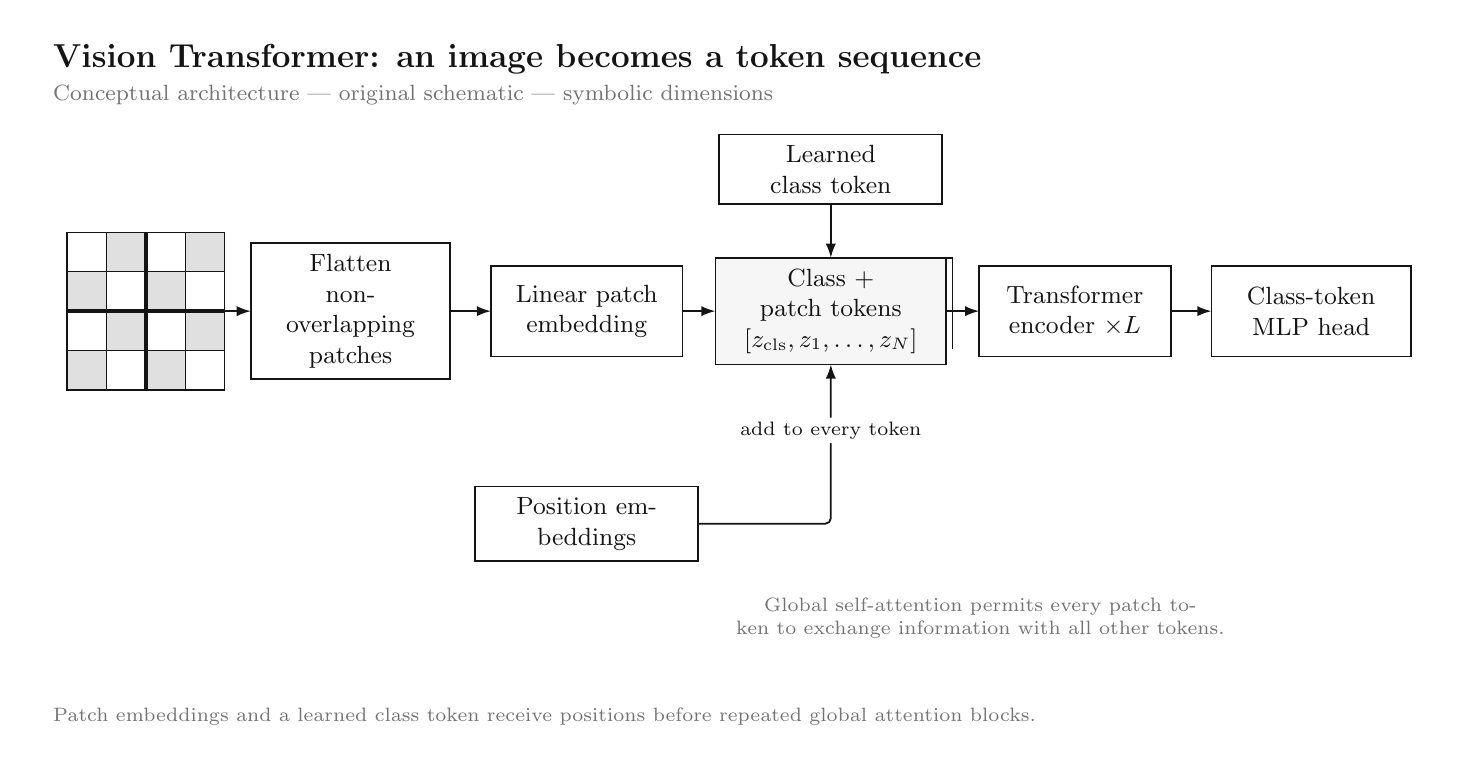
\begin{tikzpicture}[x=1cm,y=-1cm,font=\rmfamily,text=ink]

\path[use as bounding box] (0,0) rectangle (18,9);
\node[anchor=west,font=\large\bfseries] at (.2,.4) {Vision Transformer: an image becomes a token sequence};
\node[anchor=west,font=\footnotesize,text=soft] at (.2,.85) {Conceptual architecture | original schematic | symbolic dimensions};
\begin{pgfonlayer}{background}
\end{pgfonlayer}
\node[align=center,inner sep=0pt,outer sep=0pt,font=\small,minimum width=2.0cm,minimum height=2.0cm,text width=1.75cm] (image) at (1.5,3.6) {};
\node[box,minimum width=2.5cm,minimum height=1.15cm,text width=2.25cm] (patch) at (4.1,3.6) {Flatten\\non-overlapping patches};
\node[box,minimum width=2.4cm,minimum height=1.15cm,text width=2.15cm] (emb) at (7.1,3.6) {Linear patch\\embedding};
\node[box,fill=wash,minimum width=2.9cm,minimum height=1.15cm,text width=2.65cm] (seq) at (10.2,3.6) {Class + patch tokens\\$[z_{\rm cls},z_1,\ldots,z_N]$};
\draw[ink,line width=.4pt] (8.85,2.9250000000000003) -- (11.749999999999998,2.9250000000000003) -- (11.749999999999998,4.075);
\node[box,minimum width=2.4cm,minimum height=1.15cm,text width=2.15cm] (tr) at (13.3,3.6) {Transformer\\encoder $\times L$};
\node[box,minimum width=2.5cm,minimum height=1.15cm,text width=2.25cm] (head) at (16.3,3.6) {Class-token\\MLP head};
\node[box,minimum width=2.8cm,minimum height=0.7cm,text width=2.55cm] (cls) at (10.2,1.8) {Learned class token};
\node[box,minimum width=2.8cm,minimum height=0.8cm,text width=2.55cm] (pos) at (7.1,6.3) {Position embeddings};
\begin{pgfonlayer}{background}
\draw[flow] (image.east) -- (patch.west);
\draw[flow] (patch.east) -- (emb.west);
\draw[flow] (emb.east) -- (seq.west);
\draw[flow] (seq.east) -- (tr.west);
\draw[flow] (tr.east) -- (head.west);
\draw[flow] (cls.south) -- (seq.north);
\draw[flow] (pos.east) -- (10.2,6.3) -- (seq.south) node[midway,above,fill=white,inner sep=1.5pt,font=\scriptsize] {add to every token};
\end{pgfonlayer}
\fill[black!0] (0.5,2.6) rectangle (1.0,3.1);
\fill[black!12] (1.0,2.6) rectangle (1.5,3.1);
\fill[black!0] (1.5,2.6) rectangle (2.0,3.1);
\fill[black!12] (2.0,2.6) rectangle (2.5,3.1);
\fill[black!12] (0.5,3.1) rectangle (1.0,3.6);
\fill[black!0] (1.0,3.1) rectangle (1.5,3.6);
\fill[black!12] (1.5,3.1) rectangle (2.0,3.6);
\fill[black!0] (2.0,3.1) rectangle (2.5,3.6);
\fill[black!0] (0.5,3.6) rectangle (1.0,4.1);
\fill[black!12] (1.0,3.6) rectangle (1.5,4.1);
\fill[black!0] (1.5,3.6) rectangle (2.0,4.1);
\fill[black!12] (2.0,3.6) rectangle (2.5,4.1);
\fill[black!12] (0.5,4.1) rectangle (1.0,4.6);
\fill[black!0] (1.0,4.1) rectangle (1.5,4.6);
\fill[black!12] (1.5,4.1) rectangle (2.0,4.6);
\fill[black!0] (2.0,4.1) rectangle (2.5,4.6);
\draw[ink,line width=.45pt] (0.5,2.6) rectangle (2.5,4.6);
\draw[ink,line width=.45pt] (1.0,2.6) -- (1.0,4.6);
\draw[ink,line width=.45pt] (1.5,2.6) -- (1.5,4.6);
\draw[ink,line width=.45pt] (2.0,2.6) -- (2.0,4.6);
\draw[ink,line width=.45pt] (0.5,3.1) -- (2.5,3.1);
\draw[ink,line width=.45pt] (0.5,3.6) -- (2.5,3.6);
\draw[ink,line width=.45pt] (0.5,4.1) -- (2.5,4.1);
\draw[ink,line width=1.25pt] (1.5,2.6) -- (1.5,4.6);
\draw[ink,line width=1.25pt] (0.5,3.6) -- (2.5,3.6);
\node[annotation,text width=9.5cm] at (12.1,7.5) {Global self-attention permits every patch token to exchange information with all other tokens.};
\node[anchor=west,align=left,font=\scriptsize,text=soft,text width=17.6cm] at (.2,8.75) {Patch embeddings and a learned class token receive positions before repeated global attention blocks.};
\end{tikzpicture}
\end{document}
